\documentclass{article}
\usepackage[utf8]{inputenc}
\usepackage{amsmath}

\title{Przybliżenia całek oznaczonych i metody Monte Carlo}
\author{Józef Jasek}

\usepackage{natbib}
\usepackage{graphicx}

\begin{document}

\maketitle

\section{Wstęp teoretyczny}
    Omawiać będziemy 4 metody przybliżania całki oznaczonej funkcji jednej zmiennej z przedziału $[a;b]$. W drugiej części wykorzystamy metody Monte Carlo do wyznaczenia liczby $\pi$.
    \subsection{Metoda prostokątów}
    Metoda ta polega na podziale całkowanego fragmentu na $(n+1)$ równoodległych punktów. Następnie tworzymy n prostokątów, gdzie długość jednego boku to odległość między dwoma sąsiednimi punktami, a długość drugiego to f(x), gdzie x to pierwsza współrzędna drugiego wybranego punktu. Do obliczenia całki sumujemy pola utworzonych prostokątów.
    \subsection{Metoda trapezów}
    Dzielimy funkcję podobnie jak poprzednio, ale zamiast przybliżać fragmenty do prostokątów przybliżamy do trapezów i liczymy pole ze wzoru
    \[ P = h\frac{f(x_n) + f(x_{n+1})}{2} \]
    \subsection{Metoda Simpsona}
    Dzielimy funkcje podobnie jak poprzednio, ale przybliżamy fragmenty do funkcji kwadratowych i liczymy prostą całkę funkcji kwadratowej.
    \subsection{Metoda Monte Carlo}
    W tej metodzie nie stosujemy podziału na fragmenty jak poprzednio. Zamiast tego wprowadzamy zmienną losową Y z przedziału $(a;b]$ o rozkładzie jednorodnym i wykonujemy n losowań. Przybliżeniem całki jest wówczas średnie pole prostokąta o rozmiarze $f(Y)$ na $|b - a|$.
\section{Pomiary prędkości zbiegania do rozwiązania}
Wszystkie próby są wykonywane dla $n = 1000$.
    \subsection{$f_1(x) = x^2$ na przedziale $(-3;3)$}
        
        \noindent
        \makebox[\textwidth]{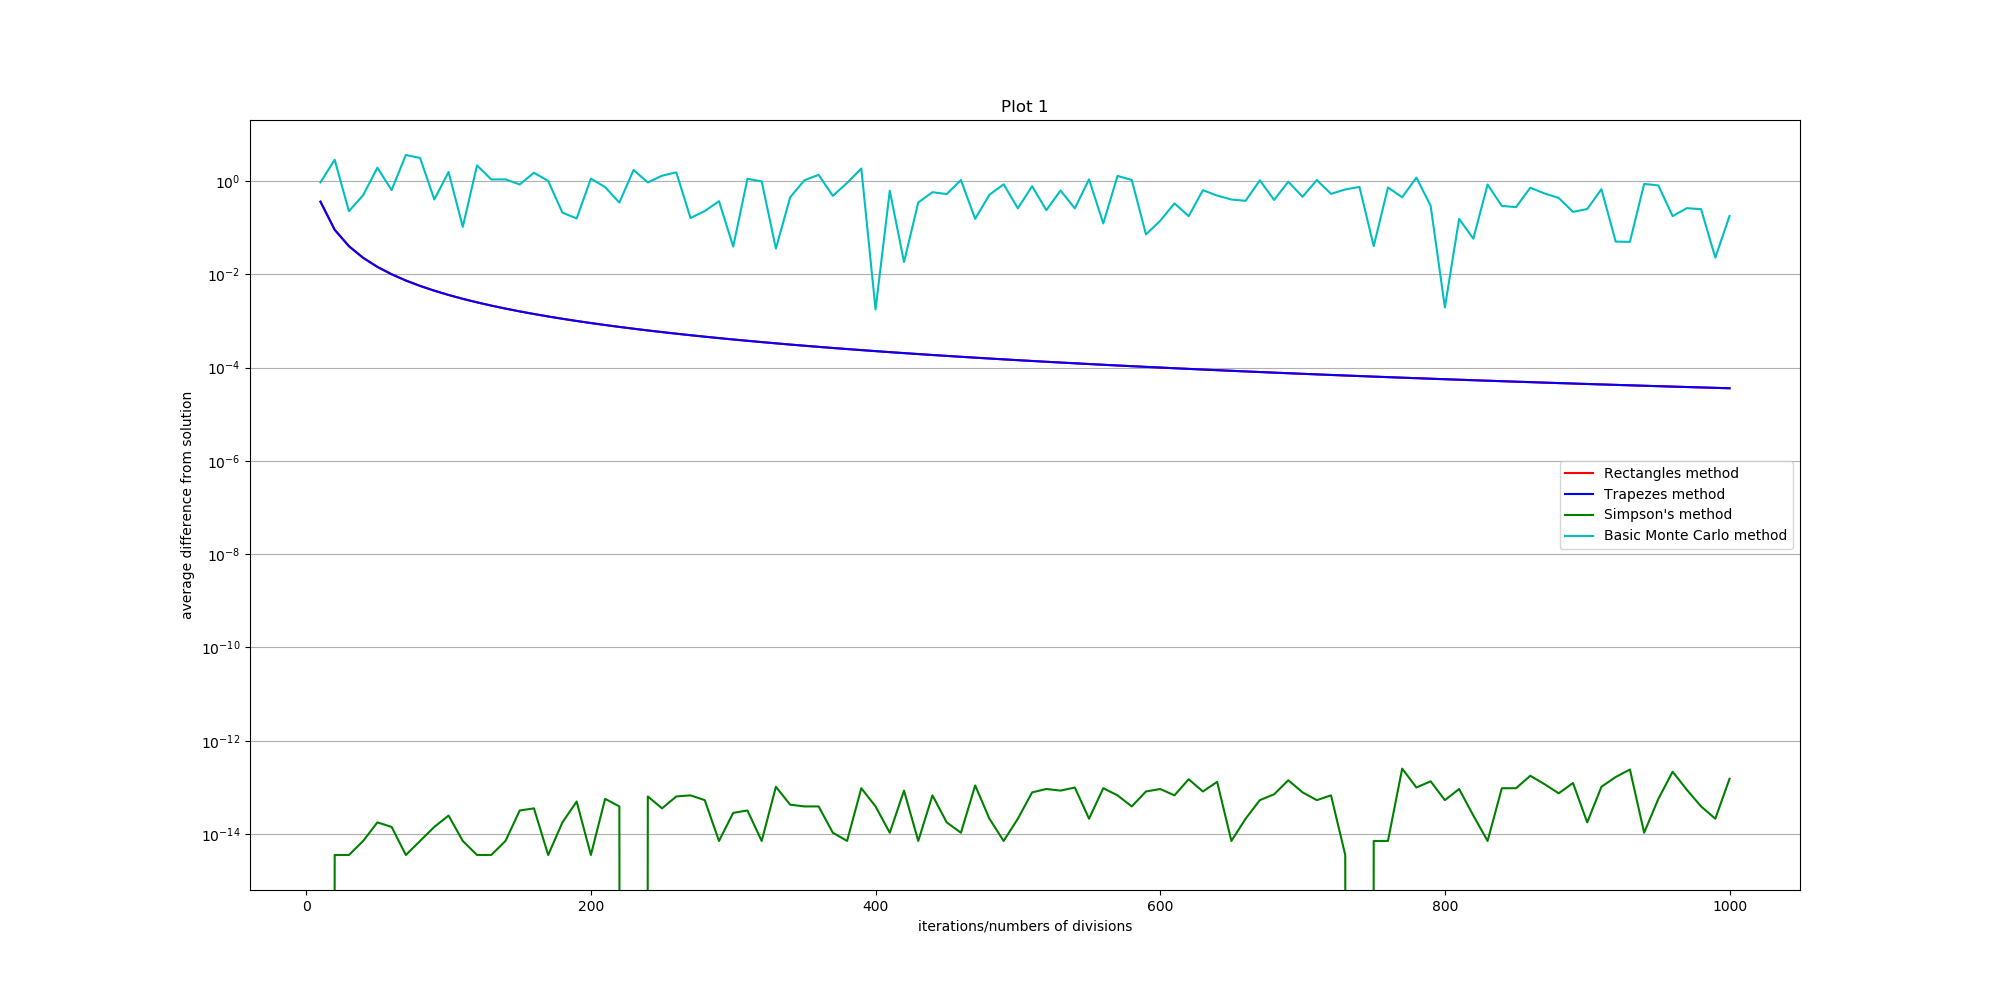
\includegraphics[width=2\textwidth]{Plot 1.png}}
    \subsection{$f_2(x) = x^3$ na przedziale $(-3;3)$}
        
        \noindent
        \makebox[\textwidth]{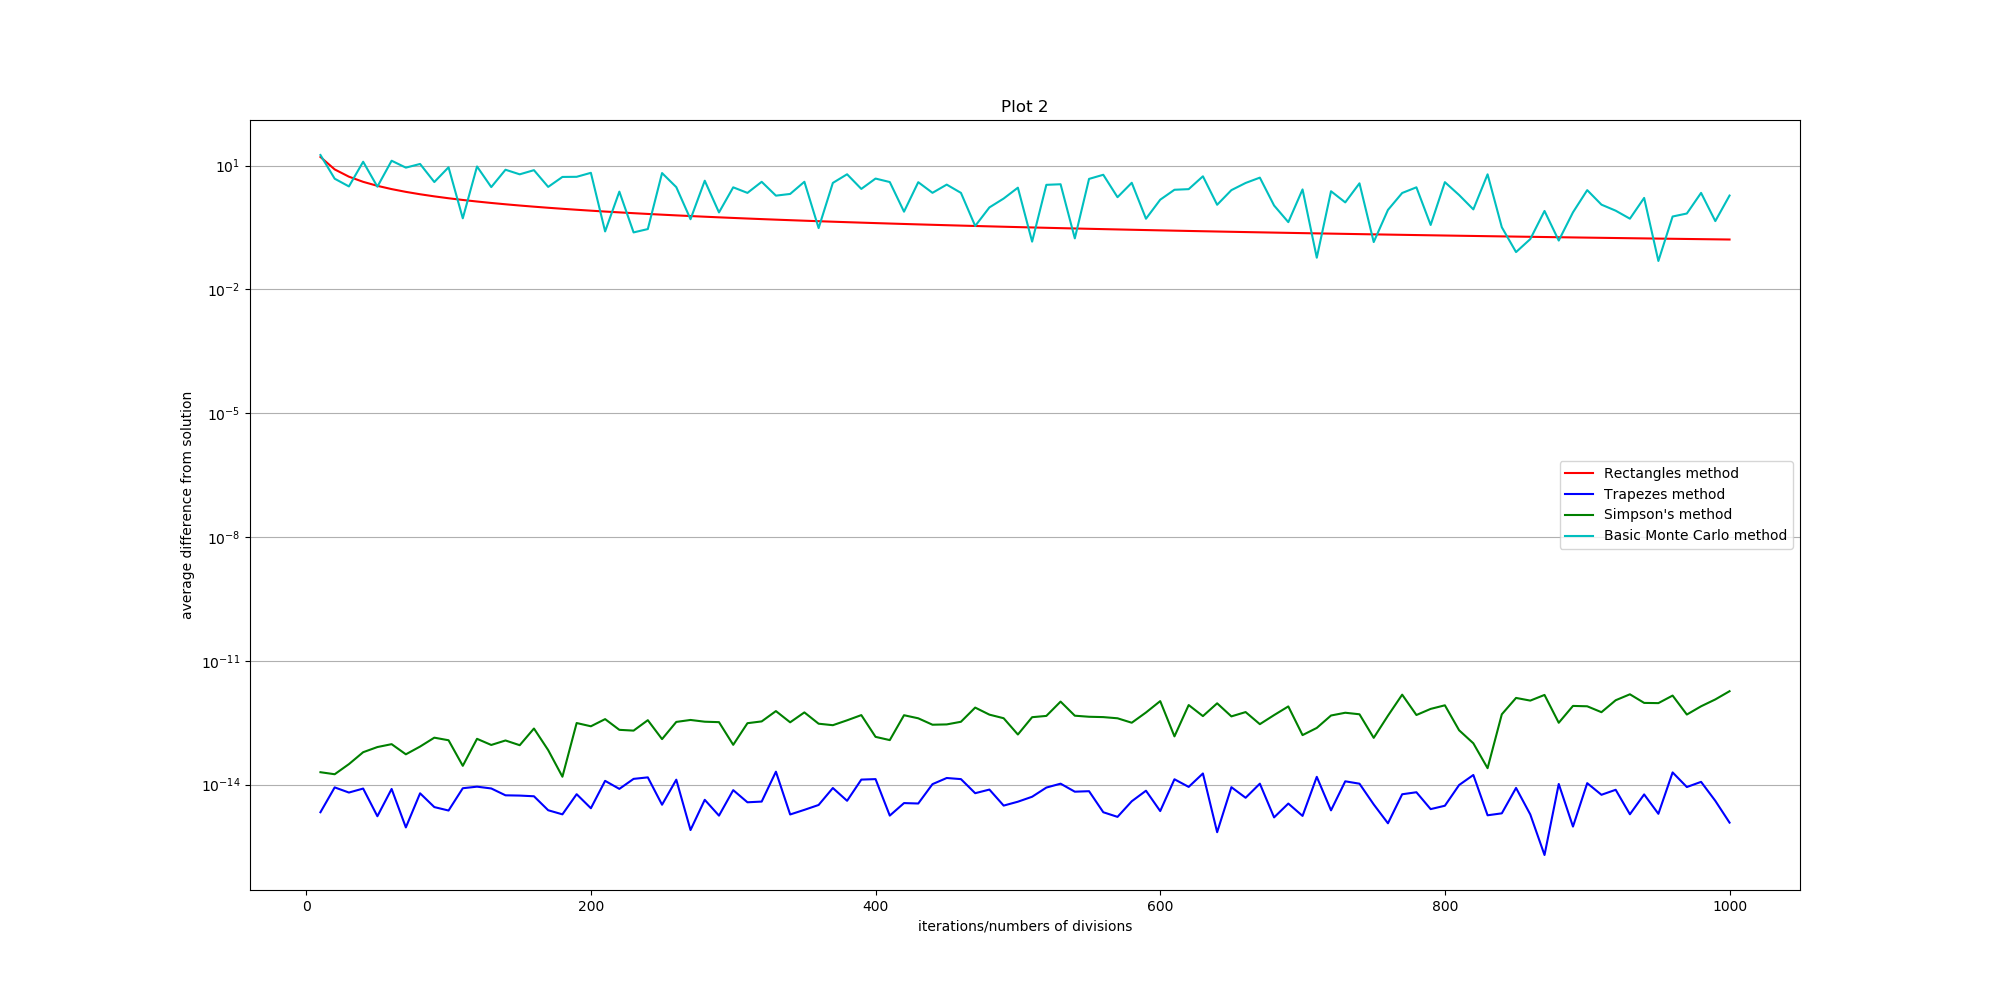
\includegraphics[width=2\textwidth]{Plot 2.png}}
    \subsection{$f_3(x) = 3x^3 - 2.34x^2 + 18x + 45$ na przedziale $(-2.6;14)$}

        \noindent
        \makebox[\textwidth]{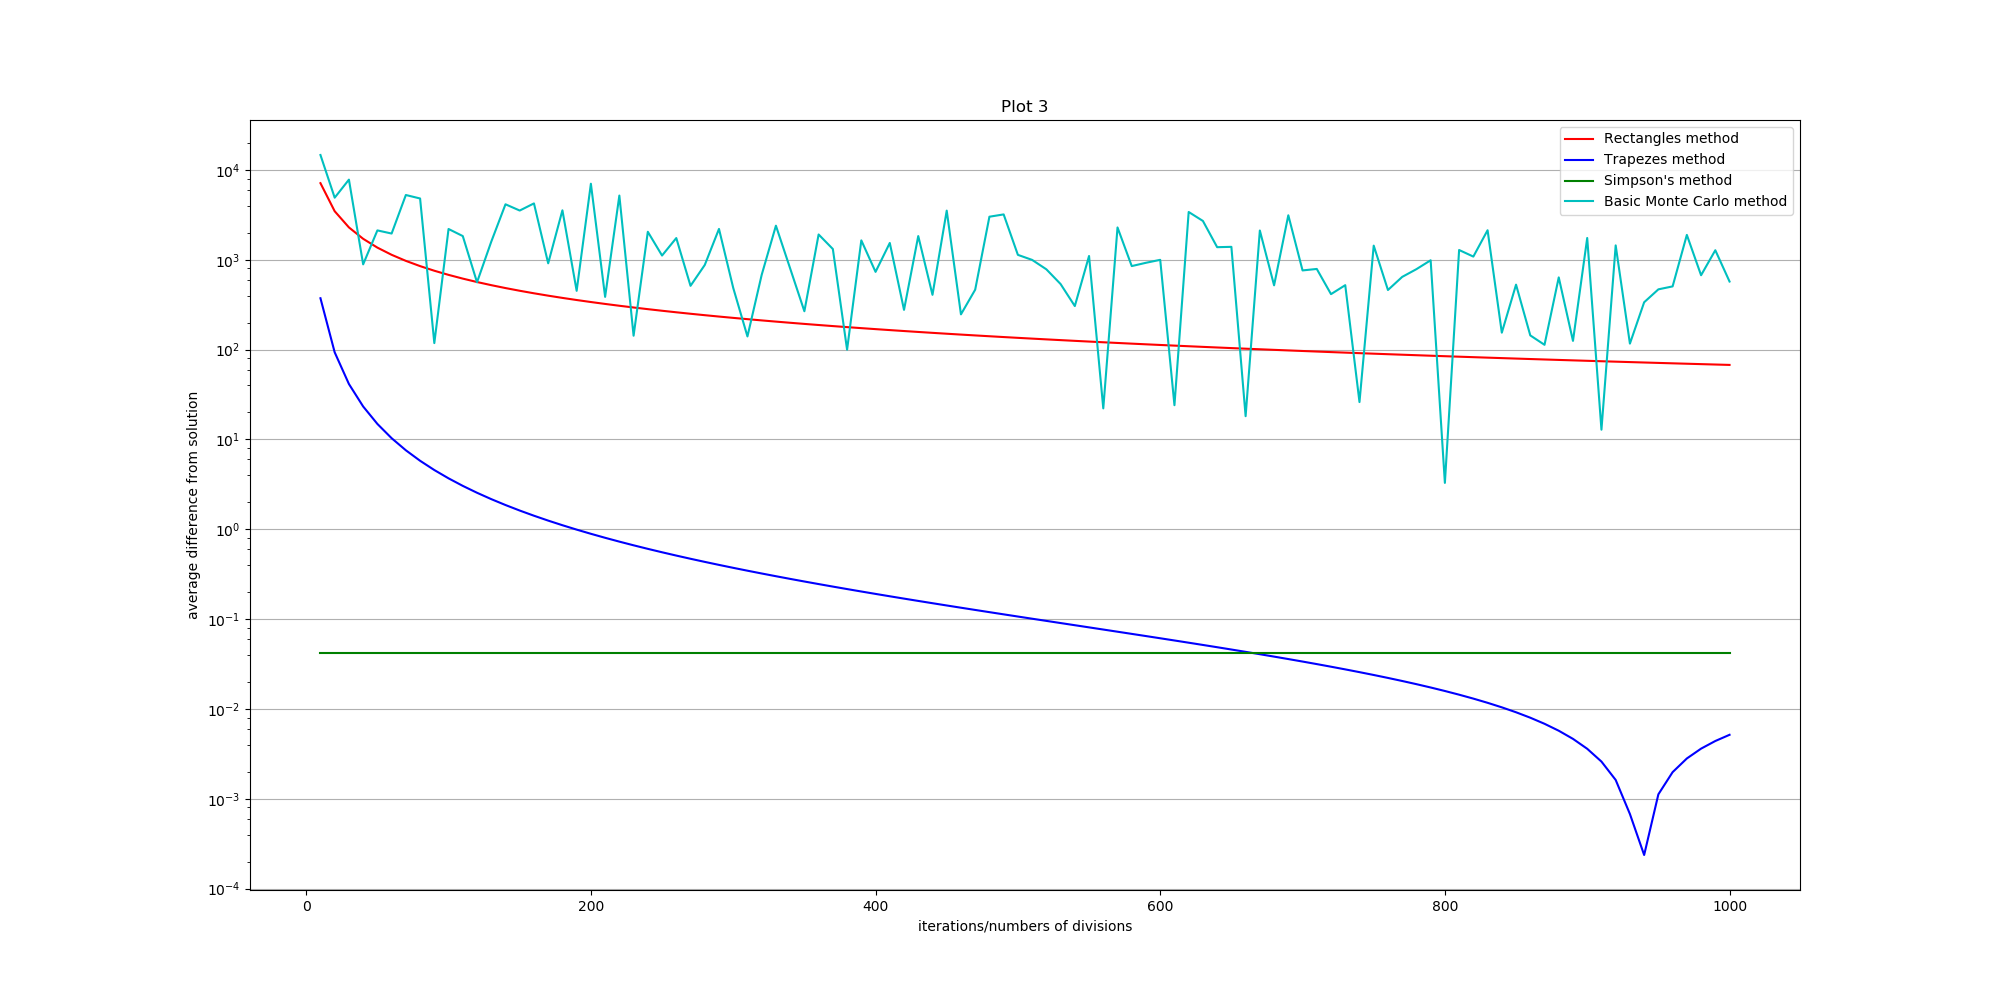
\includegraphics[width=2\textwidth]{Plot 3.png}}
    \subsection{$f_4(x) = -2x^5 + 9.21x^4 - 3.14x^3 -12x^2 + 7.2x + 15.1$ na przedziale $(-335.345; 140.82)$}

        \noindent
        \makebox[\textwidth]{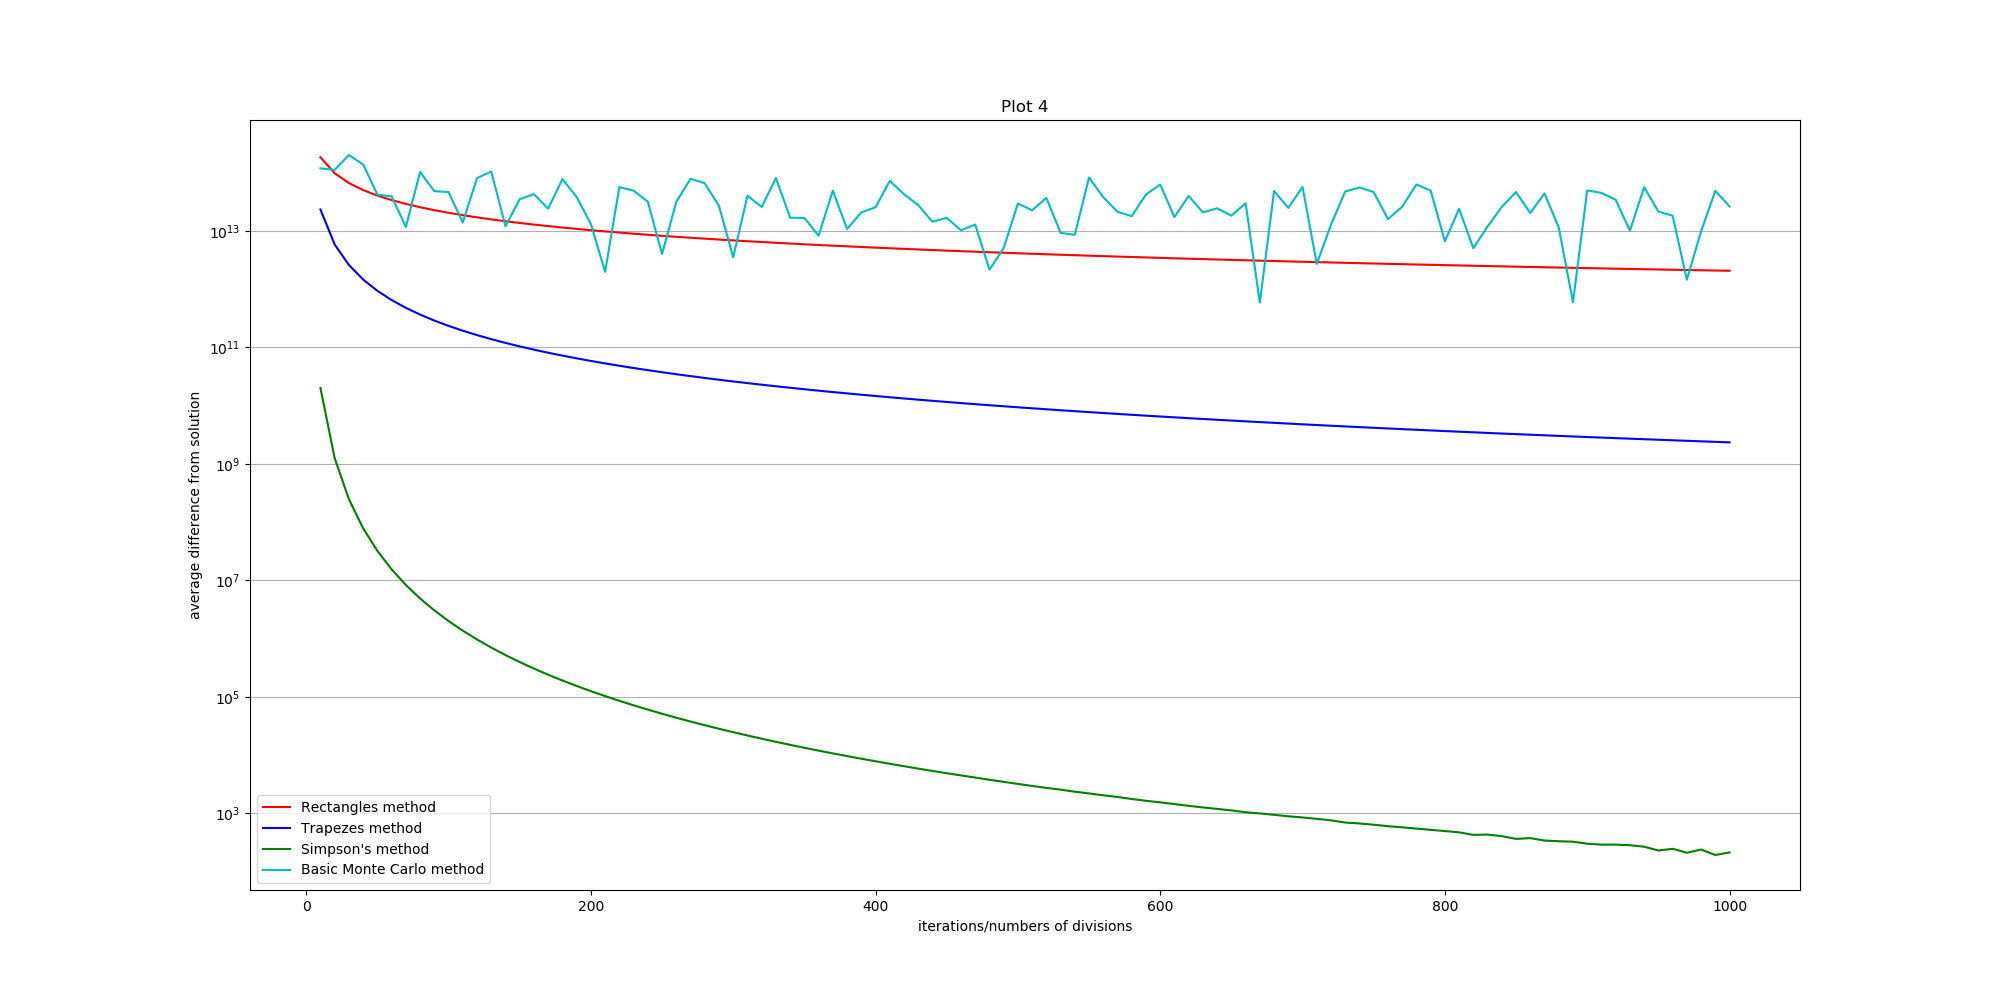
\includegraphics[width=2\textwidth]{Plot 4.png}}

\section{Wnioski}
Łatwo zauważyć, że metoda Simpsona osiąga najlepsze wyniki przy tej samej liczbie podziałów. Różnica dla ostatniej funkcji od drugiej najlepszej metody wynosi aż 7 rzędów wielkości! Widzimy też, że losowe metody Monte Carlo nie są dobrym wyborem dla tak prostych funkcji.
\section{Wyznaczanie liczby $\pi$ za pomocą metod Monte Carlo}
\subsection{Wstęp teoretyczny}
Do wyznaczenia liczby $\pi$ skorzystamy z faktu, że jeżeli pewien kwadrat zawiera jakąś figurę i wykonamy wiele rzutów w losowe miejsce wewnątrz kwadratu, to stosunek pola tej figury i pola kwadratu jest w przybliżeniu równy stosunkowi liczby rzutów, które trafiły figurę i liczby wszystkich rzutów. W naszym przypadku weźmiemy kwadrat o boku 2 i wpiszemy do niego okrąg o promieniu 1.
\subsection{Pomiary prędkości zbiegania do rozwiązania}
    \noindent
    \makebox[\textwidth]{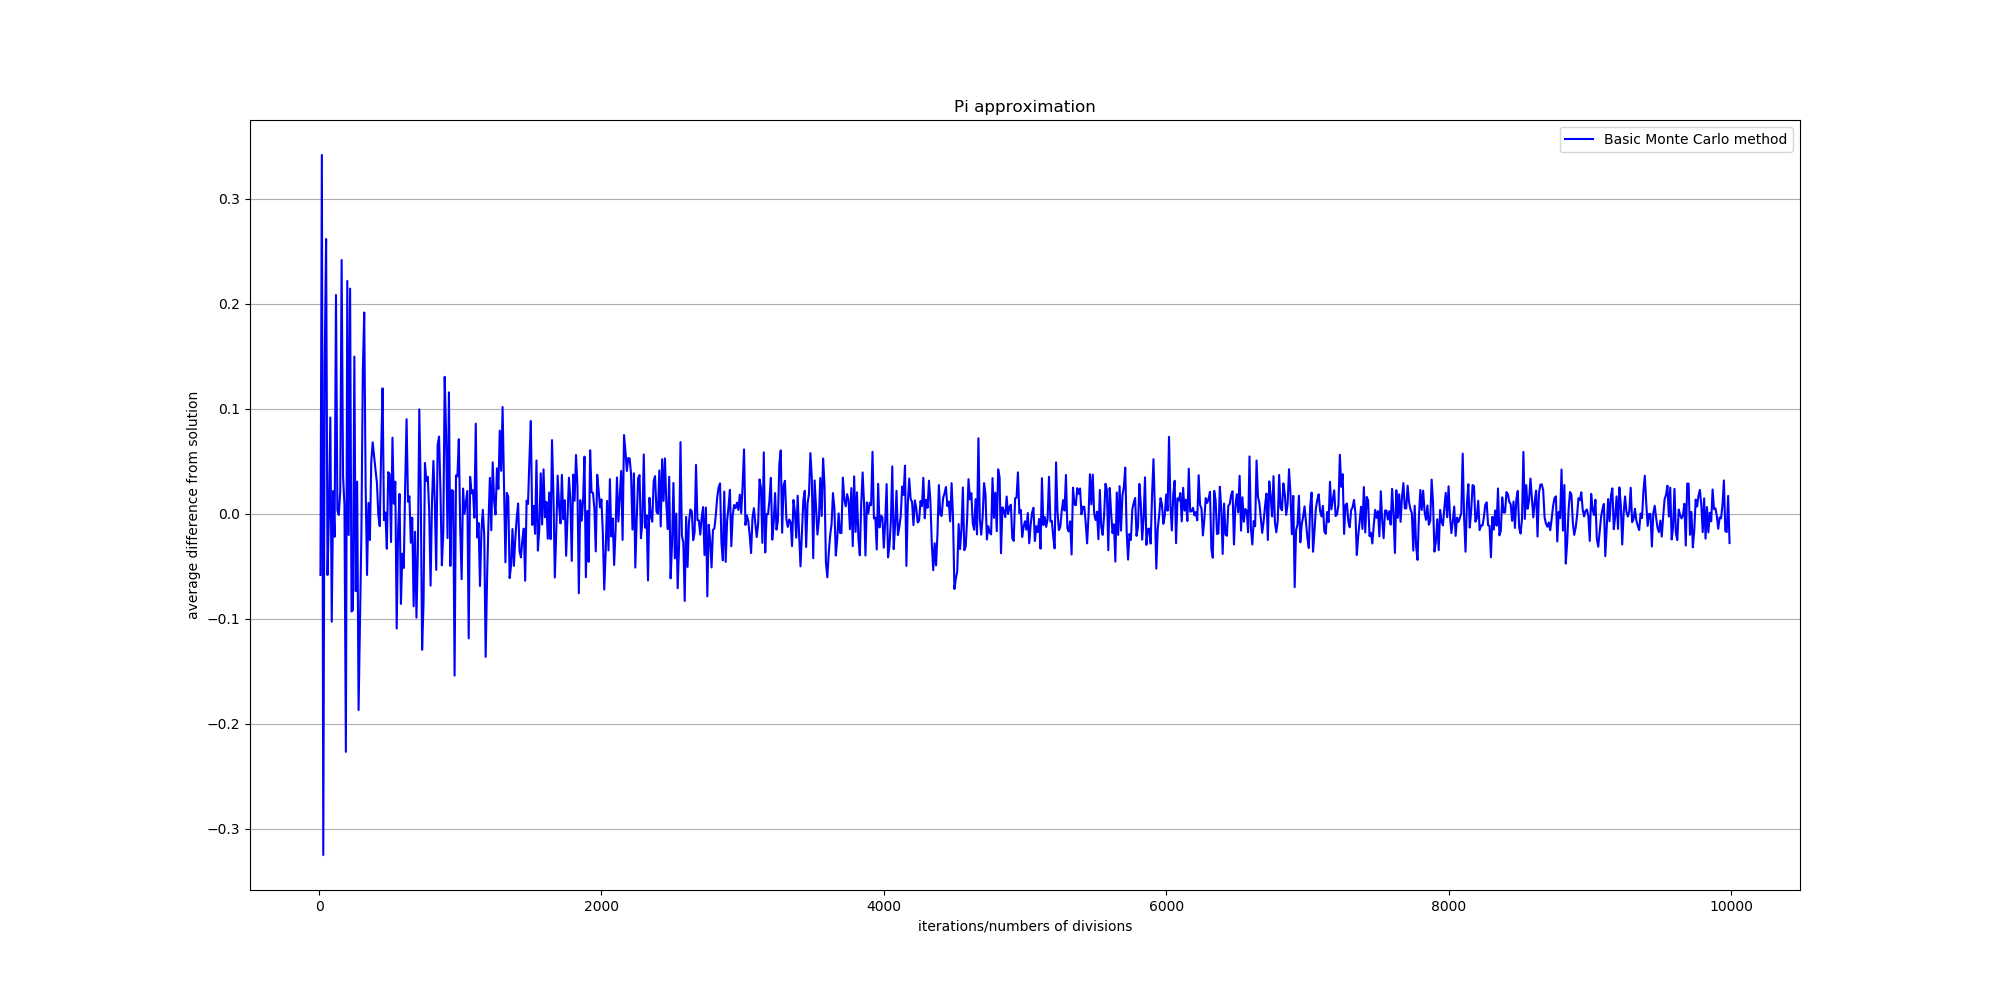
\includegraphics[width=2\textwidth]{Plot 5.png}}
\subsection{Wnioski}
Jak widać metoda pozwala wyznaczyć liczbę pi z dowolną dokładnością, ale tempo zbiegania do rozwiązania jest na tyle wolne, że nie jest to praktyczna metoda wyznaczania tej stałej.
\end{document}

